\RequirePackage{lineno}
\documentclass[a4paper,11pt]{article}
\linenumbers

\usepackage{xcolor}
%\usepackage{wrapfig}
\usepackage{graphicx}
%\usepackage{multirow}
%\usepackage{array}
%\usepackage{xspace}
%\usepackage{ifthen}
%\usepackage{times}
%\usepackage{geometry}
% \geometry{
% a4paper,
% total={170mm,257mm},
% left=15mm,
% right=15mm,
% top=30mm,
% bottom=22mm,
% }

%\usepackage{lastpage}
%\usepackage{fancyhdr}
%\pagestyle{fancy}
%\footskip 20pt
%\fancyhf{}
%\chead{Report Referee 3}
%\cfoot{{Page \thepage~of~\pageref{LastPage}}}
%\renewcommand{\headrulewidth}{0.0pt}
%\renewcommand{\footrulewidth}{0.0pt}

\begin{document}
%\fontsize{10}{12}
\selectfont


\section*{Report from referee 3 JPG}


This manuscript presents an interesting study of J/$\psi$, $\Upsilon$(1S) and $\Upsilon$(2S)
production in PbPb collisions and comparison with LHC Run-2 data by ALICE, ATLAS and CMS. 
The study is the extension to 5.02 TeV centre-of-mass energy of a similar study done for 2.76
TeV (LHC Run-1 energy) by two of the authors with a third scientist, R. Vogt, who is not author
of this manuscript. The theoretical framework combines four of the main physical effects that
are expected to contribute to the observed yield of quarkonia in PbPb collisions and to their
nucler modification factor with respect to pp collisions. Namely, initial-state nuclear shadowing,
thermal dissociation, regeneration and interaction with final-state comovers. 

My main comments and questions are the following:\newline



%Dear Editor,
%We would like to thank the referee for reviewing this paper and furnishing the report.
%We have carefully considered all comments, and we have applied the corresponding changes to the original
%version of the paper to address the issues raised. Detailed responses to all the comments made by referee
%can be found below. We are at your disposal for any further clarifications and/or additional information.

{\color{blue}
We would like to thank the referee for reviewing this paper and furnishing the report.
Detailed responses to all the comments made by referee can be found below.}


\begin{enumerate}

\item In Eq (8) the heavy quarks are assumed to be “nearly-thermalised” and their p$_T$ distribution is described by a
  Tsallis function with n=14. Can you justify this assumption? For example, does this pT shape describe the measured dN/dpT
  of D mesons in PbPb?

{\color{blue}  Here we include following revision in the paper.
    
  Since the heavy quarks produced are not fully thermalized in the medium
  we use near thermal distributions given by Tsallis function.
  (There was a typo, we used $n=12$ in the work.)
  Figure~\ref{fig:Figure2_Tsallis} gives the transverse momentum spectra of D mesons in pp and PbPb collisions
  at $\sqrt{s_{\rm NN}}=5.02$ TeV measured by CMS experiment. The spectra are fitted
  by Tsallis function with $n=6.9$ for pp and $n=12$ for PbPb collisions.
}

\begin{figure}
  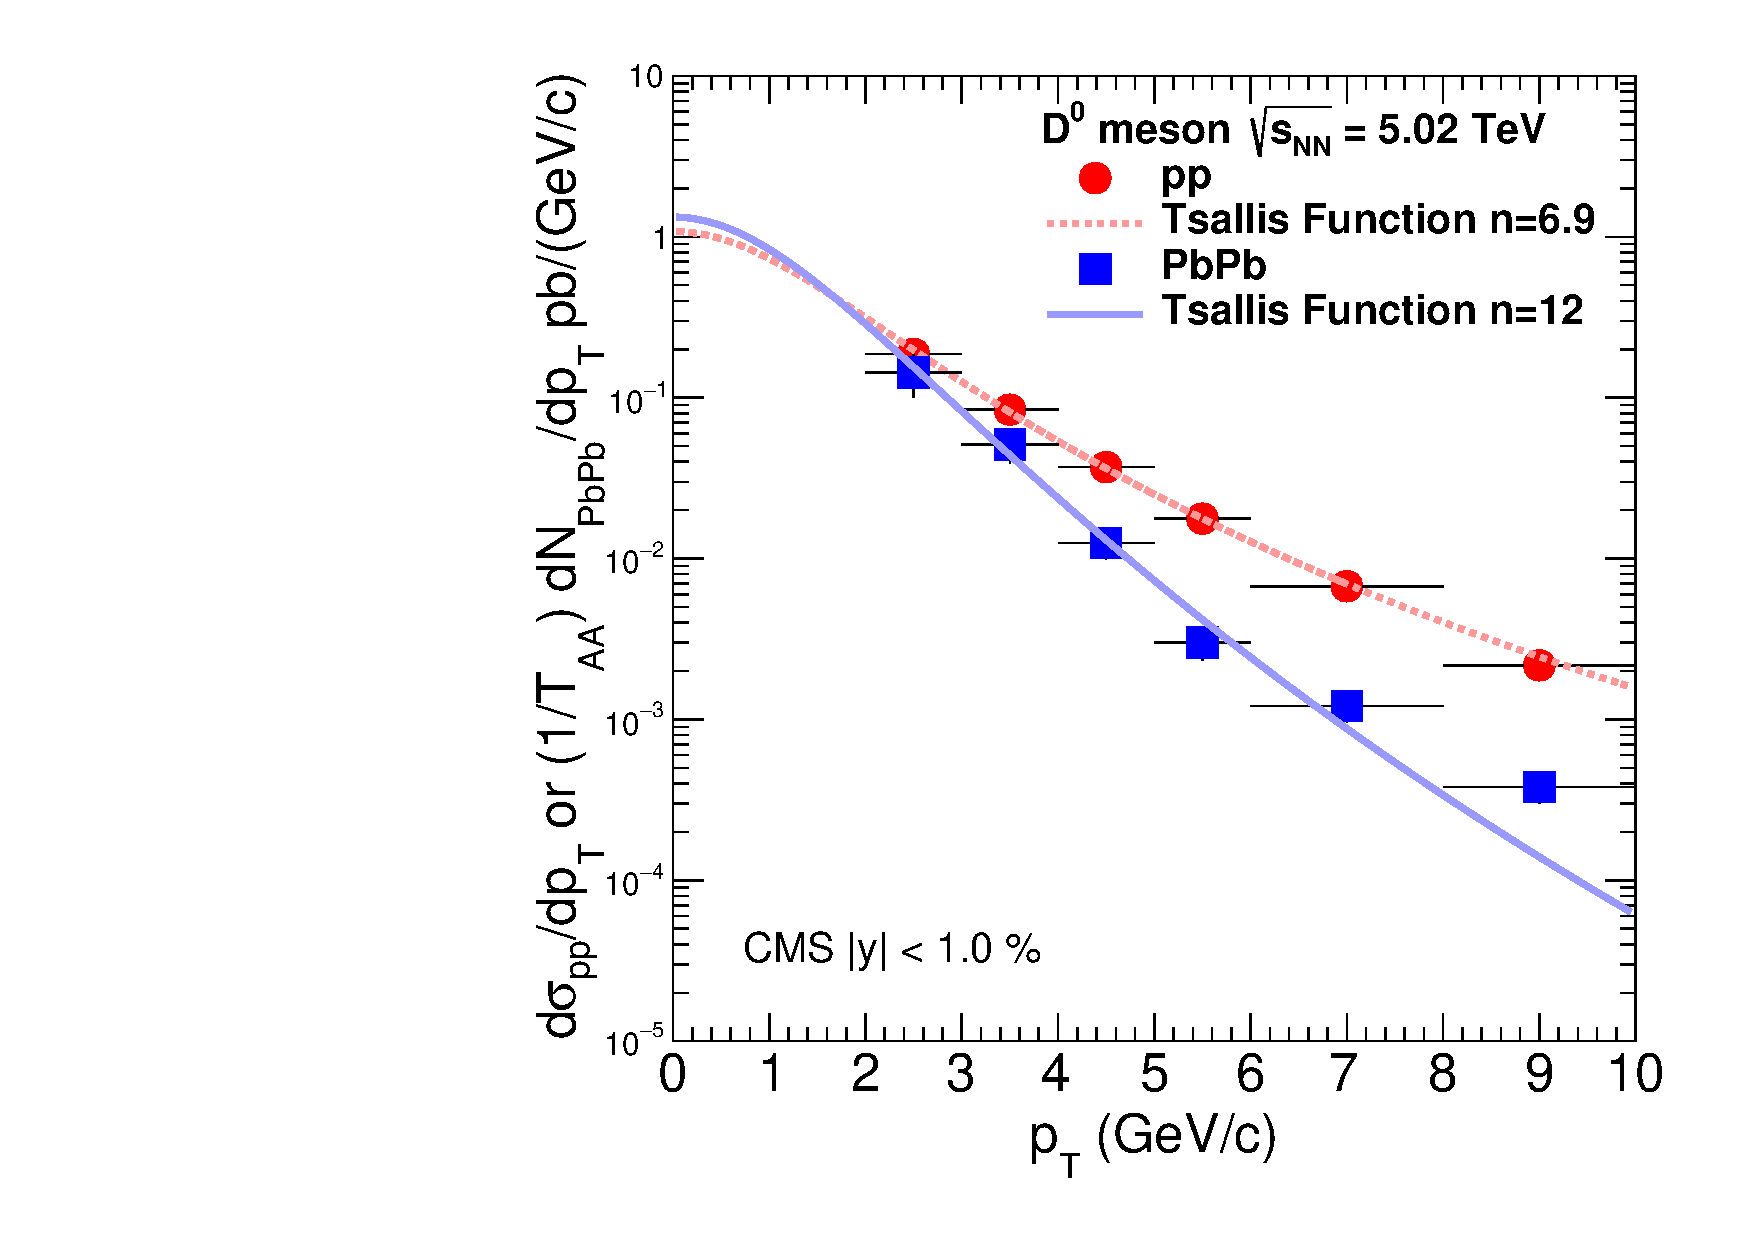
\includegraphics[width=0.60\textwidth]{Figure3_DMeson_502TeV.pdf}
  \caption{The transverse momentum spectra of D mesons in pp and PbPb collisions
    at $\sqrt{s_{\rm NN}}=5.02$ TeV measured by CMS experiment \cite{Sirunyan:2017xss}.
    The spectra are fitted
    by Tsallis function withb$n=6.9$ for pp and $n=12$ for PbPb collisions.
  }
  \label{fig:Figure2_Tsallis}
\end{figure}


\item (Related to 1), which pT distribution is assumed for quarkonia in pp collisions? This enters in the RAA versus pT

{\color{blue} The p$_T$ distribution for quarkonia in pp collisions is obtained from PYTHIA calculations. }



\item At page 7 line 48, the radius of the QGP system is parametrised as R$_A$*$\sqrt(Npart/2A)$. Please justify this assumption.\newline

  {\color{blue} This depends on the basic presumption that the overlap area $\pi R^2$ is proportional
    to the number of participants by half. In case they completely overlap the area is proportional to $A$. 
  }


\item Table 3 gives the numbers of heavy quark pairs for minimum-bias PbPb collisions. How are the values in centrality classes obtained?\newline
  
  {\color{blue} We use the number of collision scaling to obtain the number of heavy quark pairs in various centrality bins. 
    
    \begin{equation}
      N_{\rm c\overline{c}}^{\rm centbin} = \frac{N_{\rm c\overline{c}}^{\rm MB}\times N_{\rm coll}^{\rm centbin}}{N_{\rm coll}^{\rm MB}} 
    \end{equation}
  }

\item In the final curves, it would be better, in my opinion, to had in quadrature also the uncertainty band from shadowing, which is dominant at
  low pT. \newline
  {\color{blue}
    The source of uncertainty on CNM effects and hot matter effects are separated to show their relative contributions in different kinematic regions.
    As you correctly mentioned the CNM effects are more dominated in the low p$_{T}$ and forward rapidity region.  
  }


\item  The regeneration (“formation”) contribution should also be shown with an uncertainty band, including the uncertainty on the heavy quark
  cross sections, on the shadowing in PbPb and on the relevant medium parameters. Note that most of the present theoretical models of quarkonium
  producton in AA present the resulting RAA with a theoretical uncertainty band that includes these sources of uncertainty.


  {\color{blue} 
    The uncertainty has been calculated on the regeneration (“formation”) contribution using the sources
    (change in the initial time $\tau_0$ and variation of the dissociation cross-section).
    These uncertainties are then used to calculate the total uncertainty on the nuclear modification
    factor R$_{AA}$ which has been shown in all figures.
    We have not put the band on the regeneration contribution in figures but it has been included
    in the total uncertainty.}



\item It would be interesting to include also calculations for psi(2S) as well as the ratio of RAA(psi(2S))/RAA(psi(1S)), where for
  example the effect of shadowing cancels. 


  {\color{blue}
    We had been reluctant to do the calculations for $\psi$(2S) as the
    gluon dissociation cross-section for excited charmonia state is not very reliable,
    on the other hand it is usable for the bottomonia due to high mass.
  }

\end{enumerate}


- Page 1 line 42: transverse \newline
- {\color{blue} done} \newline
- Page 2 line 9: *to a* Quark Gluon Plasma \newline 
- {\color{blue} done} \newline
- Page 2 line 20: quarkonia \newline
- {\color{blue} done} \newline
- Page 2 line 35: also cite other theory works on regeneration (Thews et al, Rapp et al) \newline
- {\color{blue} done} \newline
- Page 2 line 54: remove “has” \newline
- {\color{blue} done} \newline
- Page 2 line 58: remove “on” before Jpsi; infer $\rightarrow$ show \newline
- {\color{blue} done} \newline
- Page 3 line 5: also ALICE measurements at midrapidity \newline 
- {\color{blue} done} \newline
- Page 3 line 10: J/psis $\rightarrow$ J/psi mesons \newline
- {\color{blue} done} \newline
- Page 3 line 14: where a both $\rightarrow$ where both \newline
- {\color{blue} done} \newline
- Page 3 line 17: rm “Jpsi meson” \newline
- {\color{blue} modified} \newline
- Page 3 line 34: observe*d*; is this observation statistically significant \newline
- {\color{blue} done, yes in the most central bin}\newline
- Page 3 line 37: had $\rightarrow$ has \newline
- {\color{blue} done}\newline
- Page 4 line 8: by to $\rightarrow$ by \newline
- {\color{blue} done}\newline
- Page 4 line 13: of *the* collision \newline
- {\color{blue} done}\newline
- Page 5 Eq 5: define v$_{rel}$ \newline
- {\color{blue} done}\newline

- Page 5 line 57: motivate the sqrt(Npart/2A) factor \newline
- {\color{blue} The Dissociation rate (fm$^{-1}$) is simply scaled with the relative size of the
  system. Please also see the answer in point 3.}\newline

- Page 6 line 29: how does pT enter Eq 5 \newline
- {\color{blue} The pT enters through the momentum of Quarkonia via the variable $s$
  We expand the text after Eq. 5 as;
  where $\sigma_{D}(s) = \sigma_{D}(q^0(s))$ in terms of the square of the center of
  mass energy $s$ of the quarkonium-gluon system given by
  $s=M_{Q}^{2} + 2  p_g \, \sqrt{M_{Q}^2 + p^2} - 2  p_g \, p \, {\rm cos\theta}$.
  Here $M_{Q}$ is the mass and $p$ is the momentum of quarkonium and $\theta$ is the angle
  between the quarkonium and the gluon.
}




- Page 6 line 49: in the mT formula, p should be replaced by pT. What is used in the calculation? \newline
- {\color{blue} it is p$_{T}$, the paper is modified.}\newline

- Fig 3: why is the curve decreasing with increasing T for the case of pT=3.5 GeV \newline

- {\color{blue} At higher temperature the recombined quarkonium will shift more towards higher
  $p_T$ as can be seen in Fig.3b.
}\newline




- Page 7 line 48: transverse size $\rightarrow$ radius \newline
- {\color{blue} yes}\newline

- Eq 12: it would be interesting to compare this cross section to the case of dissociation shown in Fig 1-2 \newline
- {\color{blue} As we can see from final R$_{AA}$ curves the contribution of these cross-sections is very small.
  For the more details about comover dissociation we have included reference to previous calculation~\cite{Kumar:2014kfa}.
  We are producing the dissociation cross-section in Fig.~\ref{fig:SigmaDPi}(a) and Fig.~\ref{fig:SigmaDPi}(b).
}\newline

\begin{figure}
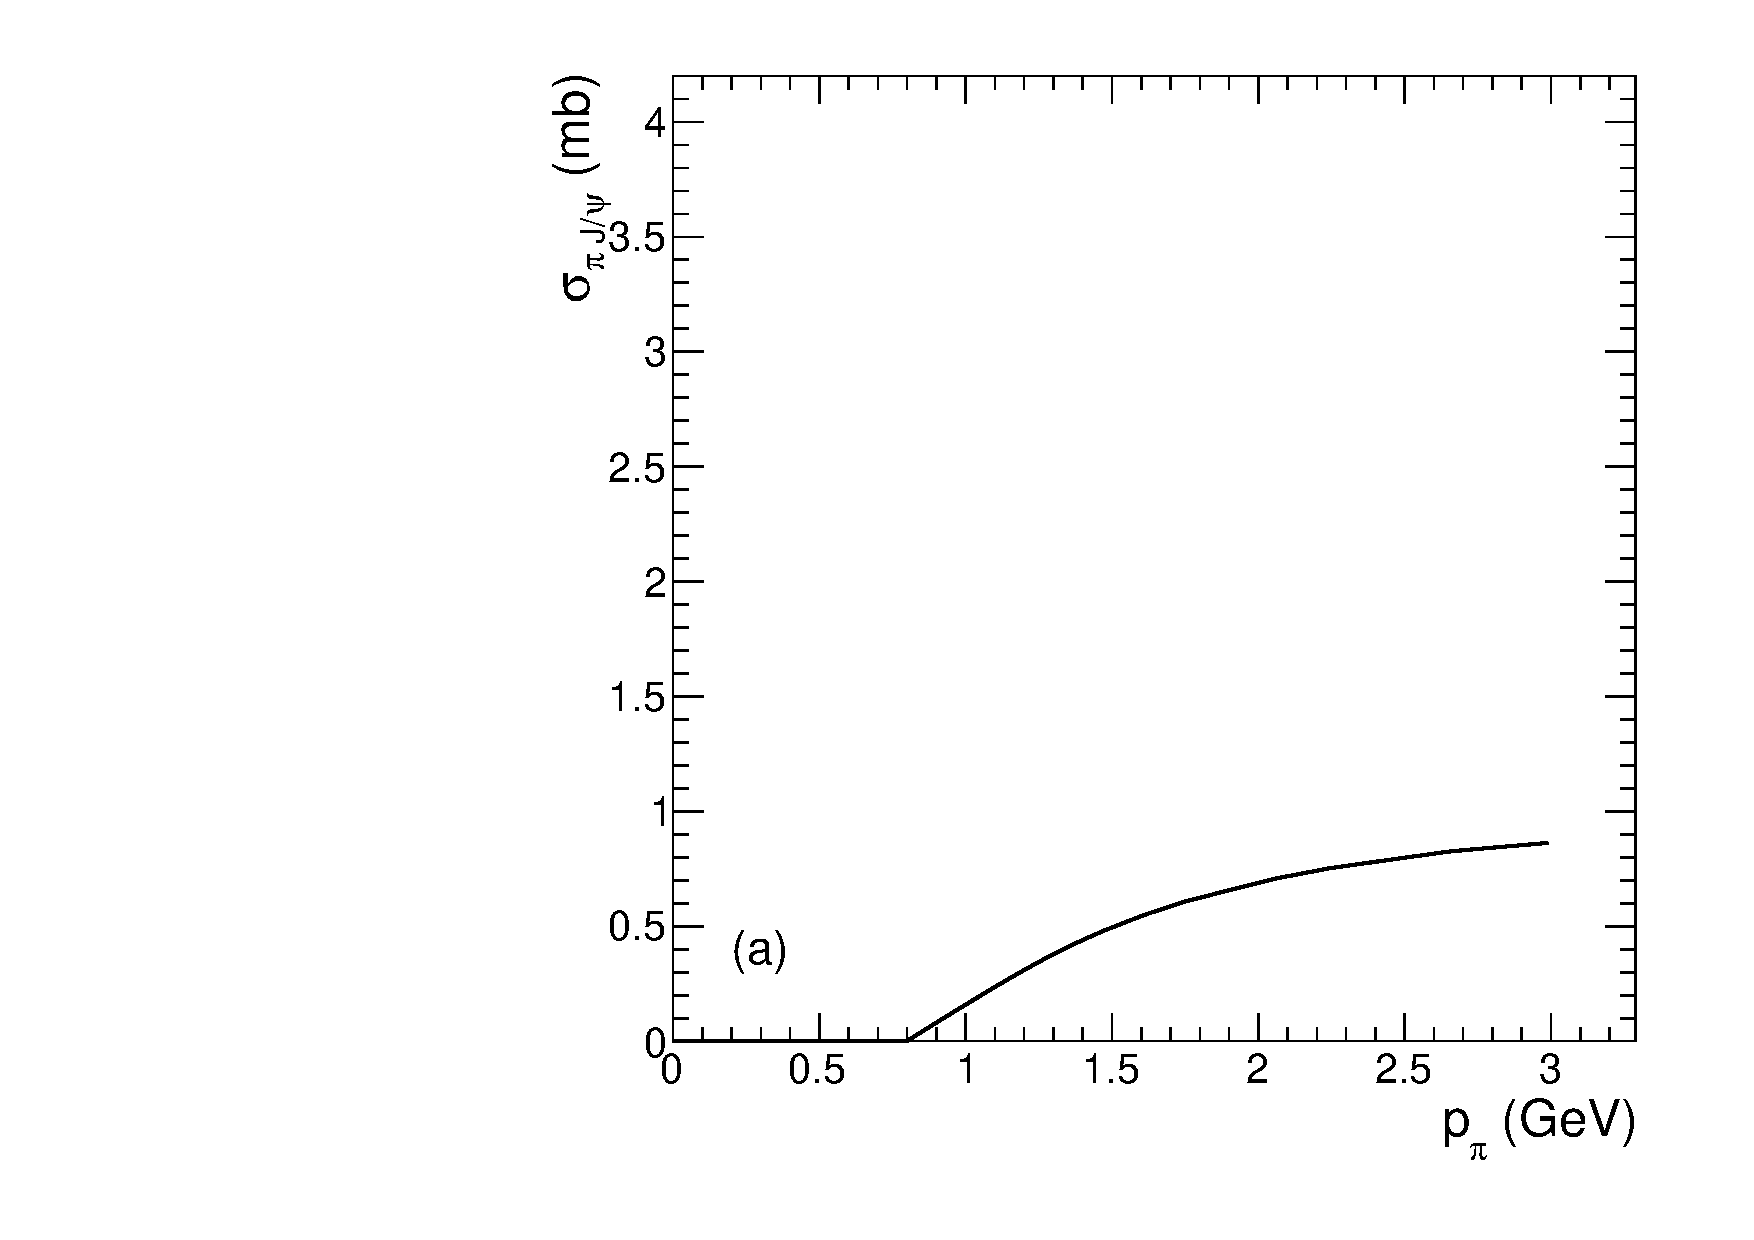
\includegraphics[width=0.49\textwidth]{Fig_JPsi_SigmaD_Pion.pdf}
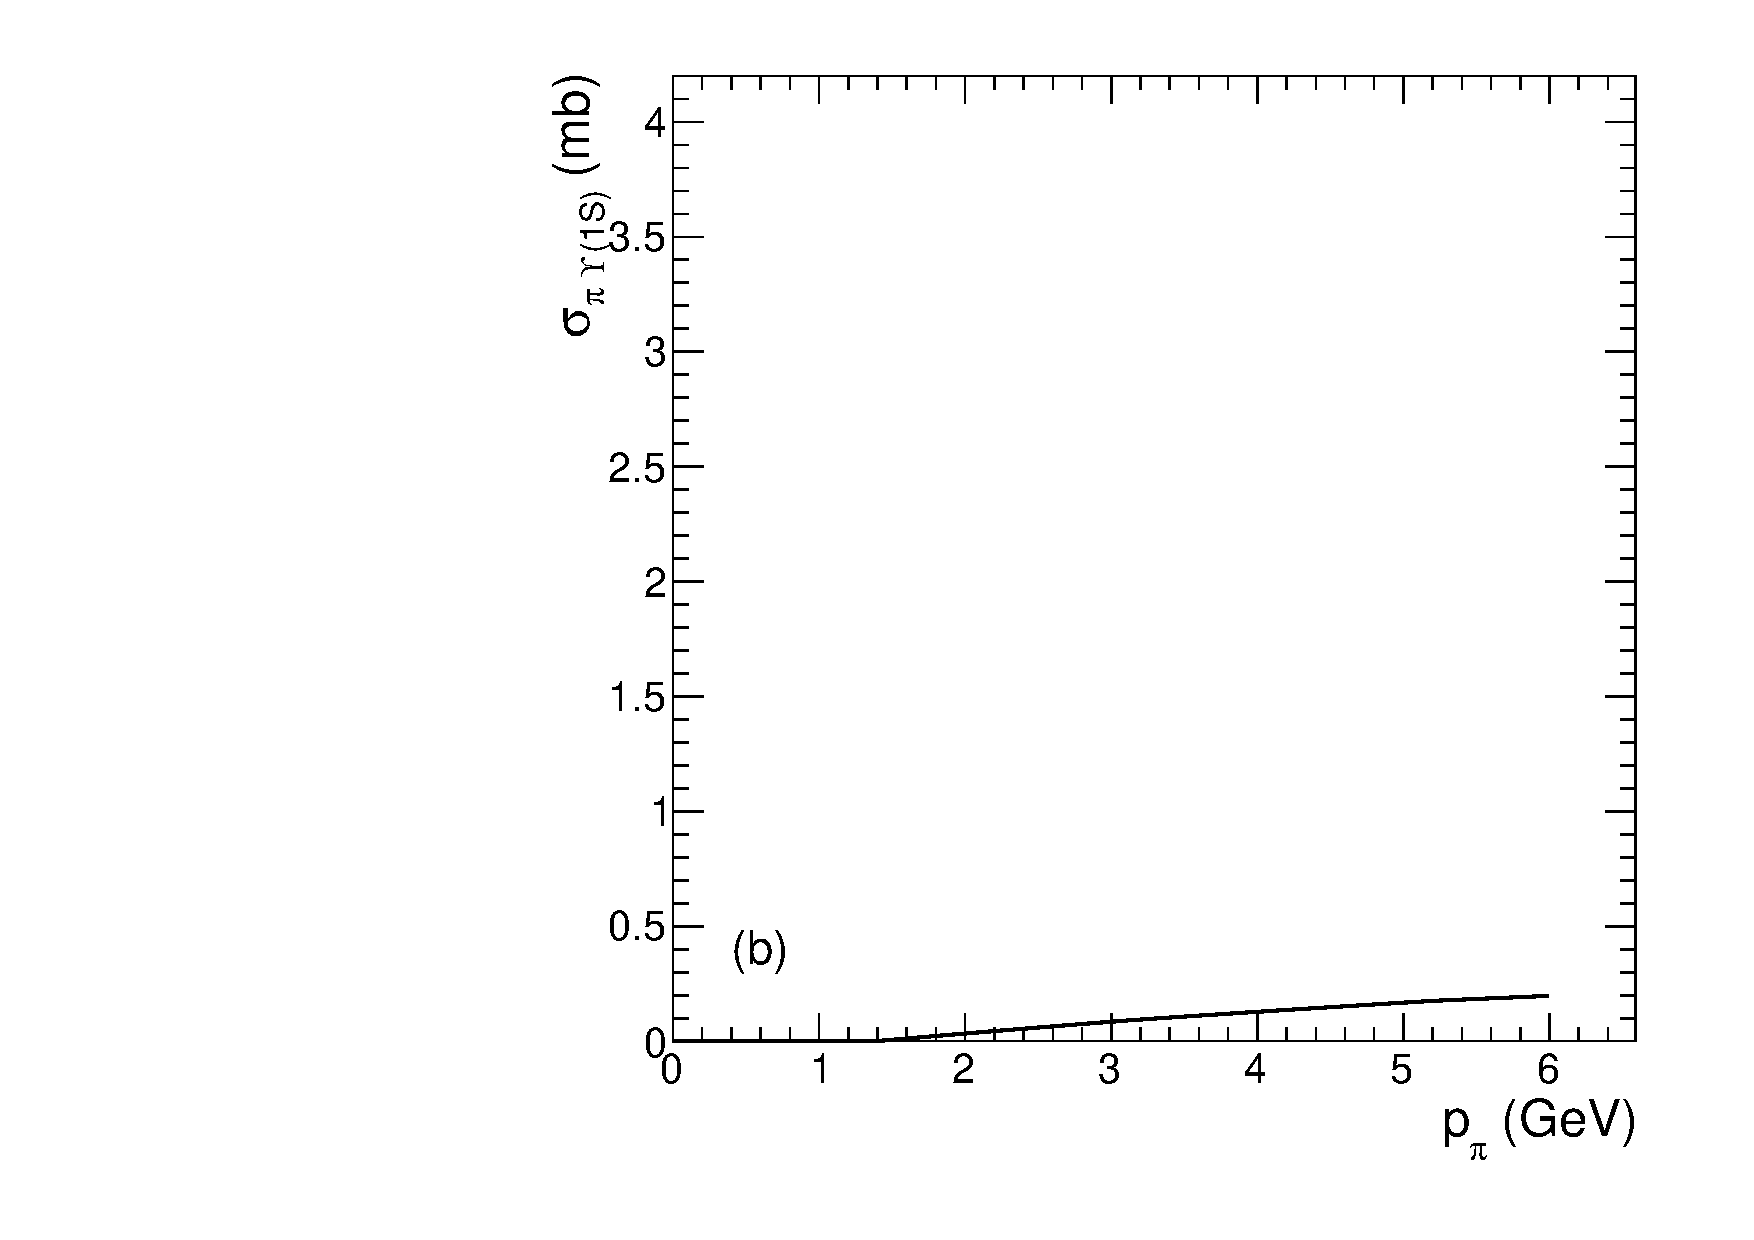
\includegraphics[width=0.49\textwidth]{Fig_Y1S_SigmaD_Pion.pdf}
\caption{Quarkonium-pion dissociation cross section cross section of J/$\psi$ (a) and $\Upsilon$(1S) (b) as a function of
pion momentum.}
\label{fig:SigmaDPi}
\end{figure}

- Tables 1 and 2: some of these measurements may be preliminary, in that case, please specify. In addition, some of these
measurements are not independent, because they use the same data samples, e.g. ALICE 52 and 53, ATLAS 54 and 55 (to be checked).
In these case, only the latest measurement/paper should be used. \newline

- {\color{red} \textbf{TBD} ??}\newline





- Page 9 line 21: quantity \newline
- {\color{blue} done}\newline

- Table 3: are these weighted means of the cross sections in tables 1 and 2? For PbPb, is nuclear shadowing included? Are the EPS09
uncertainties also included? \newline
- {\color{blue} We use the interpolation procedure to extract the cross-sections at 5 TeV. The nuclear shadowing is included in the
PbPb cross sections.}\newline

- Page 9 line 59: crucial *role* \newline
- {\color{blue} done}\newline

- In all figures with RAA data, the experimetal normalisation uncertainties at RAA=1 should also be plotted.\newline 
- {\color{blue} These uncertainties does not affect the pT and centrality distributions. We have added the
  experimetal normalisation uncertainties at R$_{AA}$=1 in the figures.}\newline

- Fig 5: are these ALICE data for 0$<$pT$<$12 or 0.3$<$pT$<$12?\newline
- {\color{blue}This is ALICE data for 0.3$<$pT$<$12.}\newline










\noindent
\begin{thebibliography}{100}
\medskip

%57



\bibitem{Sirunyan:2017xss}
  A.~M.~Sirunyan {\it et al.} [CMS Collaboration],
  ``Nuclear modification factor of D$^0$ mesons in PbPb collisions at  $\sqrt{s_\mathrm{NN}} = 5.02$ TeV,''
  Phys.\ Lett.\ B {\bf 782} (2018) 474.  [arXiv:1708.04962 [nucl-ex]].

\bibitem{Kumar:2014kfa} 
  V.~Kumar, P.~Shukla and R.~Vogt,
  ``Quarkonia suppression in PbPb collisions at $\sqrt{s_{NN}}$ = 2.76 TeV,''
  Phys.\ Rev.\ C {\bf 92}, 024908 (2015),
  [arXiv:1410.3299 [hep-ph]].


  
\end{thebibliography}







\end{document}
